\documentclass[12pt,a4paper]{article}% 

\usepackage[a4paper,margin=1in]{geometry}
\usepackage{kbordermatrix}
\usepackage{amsmath}
\usepackage{pgfplots}
\usepackage{mathtools}
\usepackage{blindtext}
\usepackage{graphicx}
\usepackage{enumitem}
\usepackage{xcolor}
\usepackage{tikz}
\usepackage{algorithm}
\usepackage{textcomp}
\usepackage[noend]{algorithmic}
\usepackage{listings}
	\lstset{
		frame=tb, % draw a frame at the top and bottom of the code block
		tabsize=4, % tab space width
		showstringspaces=false, % don't mark spaces in strings
		numbers=left, % display line numbers on the left
		commentstyle=\color{green}, % comment color
		keywordstyle=\color{blue}, % keyword color
		stringstyle=\color{red} % string color
	}

\usepackage [english]{babel}
\usepackage [autostyle, english = american]{csquotes}
\MakeOuterQuote{"}
\usepackage{pgfplots,amsmath}
\pgfplotsset{compat=1.12}



\newcommand{\TITLE}[1]{\item[#1]}
\renewcommand{\algorithmiccomment}[1]{$/\!/$ \parbox[t]{4.5cm}{\raggedright #1}}
\newbox\fixbox
\renewcommand{\algorithmicdo}{\setbox\fixbox\hbox{\ {} }\hskip-\wd\fixbox}
\newcommand{\algcost}[2]{\strut\hfill\makebox[1.5cm][l]{#1}\makebox[4cm][l]{#2}}
\usetikzlibrary{arrows,automata,positioning}
\usetikzlibrary{arrows.meta}
\usetikzlibrary{calc}

\pgfmathsetseed{3}
\newcommand*{\Comb}[2]{{}^{#1}C_{#2}}

\begin{document}
	
	
	\begin{titlepage}
	\title{
\includegraphics[width=0.38 \textwidth]{./NIT_Silchar_logo.png}\\\textbf{\large NATIONAL INSTITUTE OF TECHNOLOGY, SILCHAR}\\\textbf{{\large Department of Mathematics}}\\\bigskip {\large Project Report on,}\\\bigskip\textbf{{\normalsize "DATA TRANSMISSION ANALYSIS AND SIMULATION APPLYING AMPLITUDE/FREQUENCY MODULATION AND EFFECTS OF ATTENUATION ON THE TRANSMITTED SIGNAL." }}}
	%\author{Subject : SDC \\\\ Submitted by,\\Name : \\Scholar ID : }
	\date{\today}
	\clearpage\maketitle
	\thispagestyle{empty}
	\end{titlepage}
	
	\begin{center}
		\textbf{\large ABSTRACT}
	\end{center}
    \begin{flushleft}
    	\fontsize{12pt}{18pt}\selectfont
    	 In this project we account for and study the area of data communication, the technical aspects, theory governing the transmission of signal, simulation of different modulations, transference of the signal across the transmitting channel, effects of attenuation on the transmitting signal and finally aspects of demodulation.\\\bigskip
    	 Rigorous mathematical analysis of the different signals are done using powerful mathematical tools such as Laplace and Fourier transforms for ease of analysis of
    	 different signals as well as in application. Simulations of transmission of different kinds of signals in MATLAB are shown in this project with exquisite detail.\\\bigskip
    	 We have covered different types of modulation in theory additionally, Amplitude and Frequency in particular for this project. The process of modulation with carrier signal
    	 and input/message signal is examined thoroughly.\\\bigskip
    	 We try to cater to the power of computer software such as MATLAB, open source software such as \LaTeX to develop this project.
	\end{flushleft}
	
	\pagebreak
	\tableofcontents
	\cleardoublepage
	\section{Introduction}\label{sec:intro}
	\begin{flushleft}
		\subsection{Types of Data Communication}
		\begin{flushleft}
			content...
		\end{flushleft}
		\subsection{Model of Communication}
		\begin{flushleft}
			content...
		\end{flushleft}
		\subsection{Modes of Communication}
		\begin{flushleft}
			content...
		\end{flushleft}
		\subsection{Techniques of Communication}
		\begin{flushleft}
			content...
		\end{flushleft}
	\end{flushleft}
	\pagebreak
	\section{Modulation}
	
	\begin{flushleft}
		\subsection{Need of Modulation}
		\begin{flushleft}
			content...
		\end{flushleft}
		\subsection{Antenna Theory}
		\begin{flushleft}
			content...
		\end{flushleft}
		\subsection{Types of Modulation}
		\begin{flushleft}
			content...
		\end{flushleft}
		\subsection{Modulation Process}
		\begin{flushleft}
			content...
		\end{flushleft}
		\subsection{Modulation Process}
		\begin{flushleft}
			content...
		\end{flushleft}
	\end{flushleft}
	\pagebreak
	\section{Amplitude Modulation(AM)}
	\begin{flushleft}
		\subsection{Introduction}
		\begin{flushleft}
			Amplitude Modulation is a modulation technique in which the amplitude of another signal called \textit{carrier signal} $c(t)$ is varied in accordance with the \textit{message/input/modulating signal} $m(t)$. The modulating signal or $m(t)$ contains the intended message or information that is to be transmitted across the channel. The modulating signal contains the intended message or information sometimes consisting of audio data, as for an example in \textit{AM} radio broadcasting, or two-way radio communications.
		\end{flushleft}
		\subsection{Modulation Process}
		\begin{flushleft}
			The high-frequency sinusoidal waveform(i,e., \textit{carrier signal}) is modulated with respect to the input signal by combining it with the message signal using a \textit{multiplier} or \textit{mixer}. It is worth mentioning that mixing is a non-linear operation because it generates new frequencies. An example of visual realization of Amplitude modulation is shown as follows:
			\begin{center}
				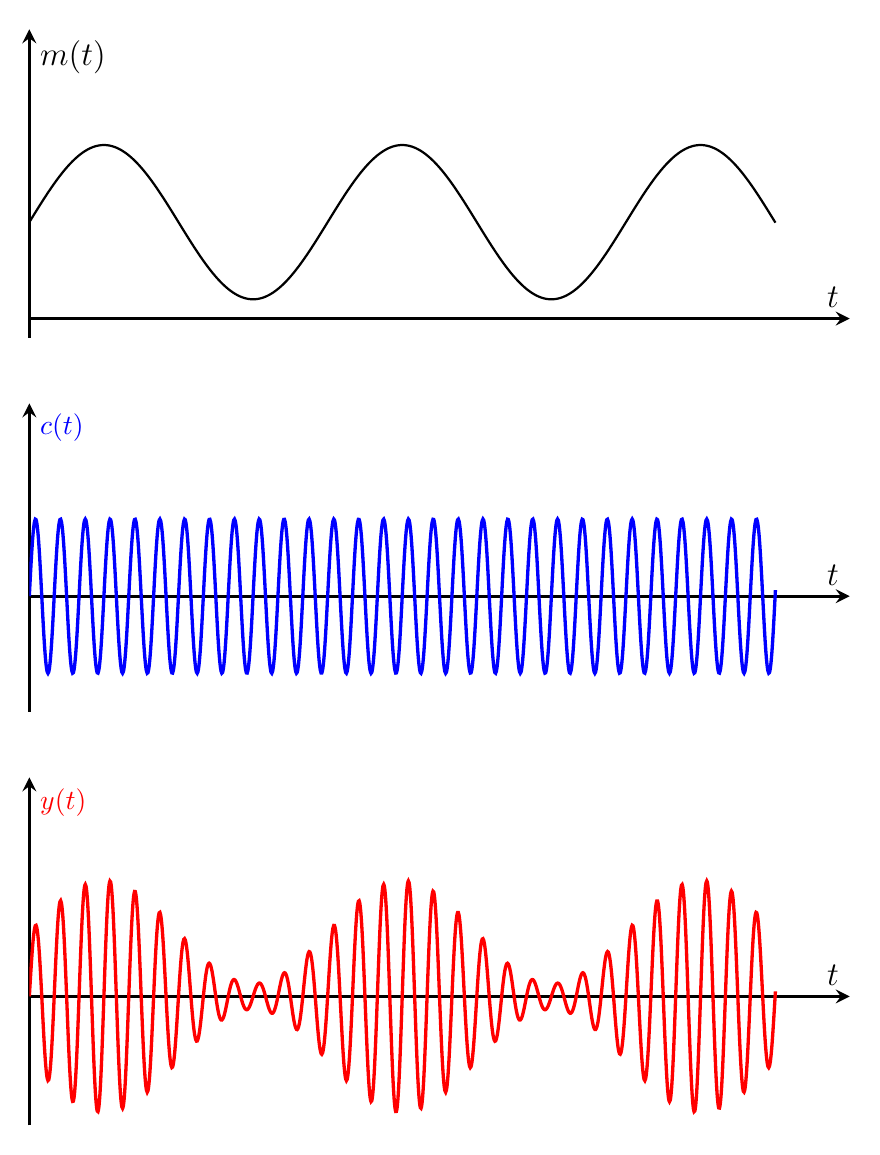
\begin{tikzpicture}[samples=1000, domain=0:10*pi]
				
				\begin{axis}[
				width=12cm, height=5.5cm,
				xtick=\empty,
				ytick=\empty,
				xlabel={\large $t$},
				ylabel={\large $m(t)$},
				xmin=0, xmax=11*pi,
				ymin=-0.5, ymax=7.5,
				axis lines = middle,
				very thick,
				trig format = rad
				]
				\addplot [no markers, smooth, thick] {2.5 + 2*sin(0.5*x)};
				\end{axis}
				
				\begin{axis}[
				at={(0, -4.75cm)},
				width=12cm, height=5.5cm,
				xtick=\empty,
				ytick=\empty,
				xlabel={\large $t$},
				ylabel={\textcolor{blue}{$c(t)$}},
				xmin=0, xmax=11*pi,
				ymin=-3, ymax=5,
				axis lines = middle,
				very thick,
				trig format = rad
				]
				\addplot [no markers, smooth, blue, very thick] {2*sin(6*x)};
				\end{axis}
				
				\begin{axis}[
				at={(0, -10cm)},
				width=12cm, height=6cm,
				xtick=\empty,
				ytick=\empty,
				xlabel={\large $t$},
				ylabel={\textcolor{red}{$y(t)$}},
				xmin=0, xmax=11*pi,
				ymin=-10, ymax=17,
				axis lines = middle,
				very thick,
				trig format = rad
				]
				\addplot [no markers, smooth, red, very thick] {(2.5 + 2*sin(0.5*x)) * 2*sin(6*x)};
				\end{axis}
				\end{tikzpicture}
			\end{center}
			\begin{center}
				The signal in red \textit{i.e.,} $y(t)$ is the \textit{amplitude modulated} wave.
			\end{center}
		Generally we have the modulated signal as $y(t)=m(t).c(t)$, but in case of amplitude modulation if we use this form, there is a serious problem of phase reversal \textit{i.e.,} the signal crosses the $x-axis$, which in turn when multiplication causes the problem of phase reversals.
		\end{flushleft}
		\begin{center}
			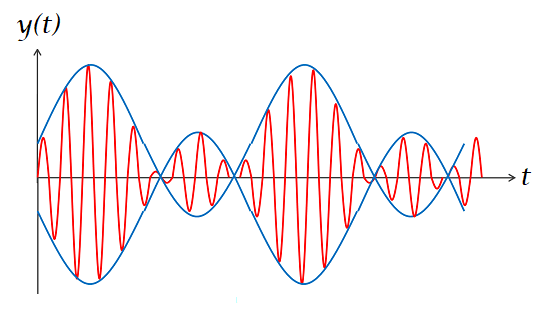
\includegraphics[width=0.60 \textwidth]{./SDC-Phase Reversal_1.png}
		\end{center}
		The mechanism of retrieval of original message signal from such a phase reversed signal is complicated and impractical for implementation. So, we improvise and solve this problem.\\\smallskip
		To do so, we shift our message signal $m(t)$, by some \textit{DC} value say $A$ and then multiply it with its carrier signal, for modulation purposes.\\\smallskip
		The general form of such signal is given by the following equation,
		\begin{equation}
			y(t)=A_c [1+k_a m(t)]cos(2 \pi f_c t)
		\end{equation}
		From the above equation if we observe then, the message signal is measured in $volts$. Therefore, by dimensional analysis the unit of $k_a$ is $volts^{-1}$.So,\\\smallskip
		$k_a$, is the amplitude sensitivity.\\
		$m(t)$ is the message/modulating signal.\\
		$y(t)$ is the modulated wave.\\\smallskip
		The \textit{envelope} of $y(t)$ in particular has same shape as the baseband signal $m(t)$ provided that the following two requirements are satisfied,
		\begin{itemize}
			\item{
				The amplitude of $k_a m(t)$ represented as $|k_a m(t)|$ is always less than unity,\textit{i.e.,}
				\begin{equation}
					|k_a m(t)| \leq 1,\enspace \forall \enspace t
				\end{equation}
				\begin{itemize}
					\item{It ensures that the function $1+k_a m(t)>0$, and since an envelope is positive. We can represent it as $A_c [1+k_a m(t)]$.}
					\item{When, $|k_a m(t)|>1$, $y(t)$ becomes overmodulated, resulting in carrier phase reversals whenever the factor as mentioned $1+k_a m(t)$ crosses zero.
					\item{The absolute maximum value of $k_a m(t)$ multiplied by $100$ is referred to as \textit{percentage modulation}}}
				\end{itemize}
			}
			\item{
				The carrier frequency $f_c$ is much greater than the highest frequency component $W$ of the message signal $m(t)$\textit{i.e.,}
				\begin{equation}
					f_c \gg W
				\end{equation}
				\begin{itemize}
					\item{If the above condition is not satisfied, an envelope cannot be realized successfully. The component $W$, is called the message bandwidth.}
				\end{itemize}
			}
		\end{itemize}
		
		If we take the \textit{fourier} transform of \textit{equation} (), then we have,
		
		\begin{center}
		$$F(y(t))=Y(f)=\int_{-\infty}^{\infty} A_c [1+k_a m(t)]cos(2 \pi f_c t) dt$$\\\smallskip
			\begin{flushleft}
				Upon, using the following results we simplify the above equation,\\\smallskip
			\end{flushleft}
			\begin{itemize}
				\item{$cos(x)=\dfrac{e^x-e^{-x}}{2}$}
				\item{$\int_{-\infty}^{\infty} e^{j 2 \pi f (t-a)} df=\delta (t-a)=\delta (a-t)$}
			\end{itemize}
			
		\end{center}
		We find that,
		\begin{equation}
			F(cos(2 \pi f_c t))=\dfrac{\delta(f-f_c)+\delta(f+f_c)}{2}
		\end{equation}
		\textit{equation} $Y(f)$ implies,
		\begin{equation}
		Y(f)=\dfrac{A_c}{2}[\delta(f+f_c)+\delta(f-f_c)]+\dfrac{k_a A_c}{2}[M(f+f_c)+M(f-f_c)]
		\end{equation}
		\subsection{Types of Amplitude Modulation}
		\begin{flushleft}
			\begin{itemize}
				\item{\textbf{Double Side Band - with Carrier(DSB-WC)} : This form of Amplitude Modulation is most widely used. All radio channels in the AM band use this type of modulation.}
				\item{\textbf{Double Side Band - Suppressed Carrier(DSB-SC)} : This form of Amplitude Modulation is same as the above mentioned except for the fact that it is without carrier(\textit{suppressed}).}
				\item{\textbf{Single Side Band (SSB)} : In this form of AM the only half of the signal of DSB-SC is used.}
				\item{\textbf{Vestigial Side Band (VSB)} : This is the modified version of SSB, to ease the generation and reception of the signal.}
			\end{itemize}
		\end{flushleft}
		\subsection{Advantages}
		\begin{flushleft}
			conten
		\end{flushleft}
	\end{flushleft}
	\pagebreak
	\section{Frequency Modulation}
	\pagebreak
	\section{Experimentation}
	\pagebreak
	\section{Simulation}
	\pagebreak
	\section{Code}
	\pagebreak
	\section{Attenuation}
	\pagebreak
	\section{Demodulation}
	\pagebreak
 	
\end{document}